\definecolor{exampleJzero}{RGB}{0,114,178}
\definecolor{exampleJone}{RGB}{213,94,0}
\definecolor{exampleJtwo}{RGB}{0,158,115}
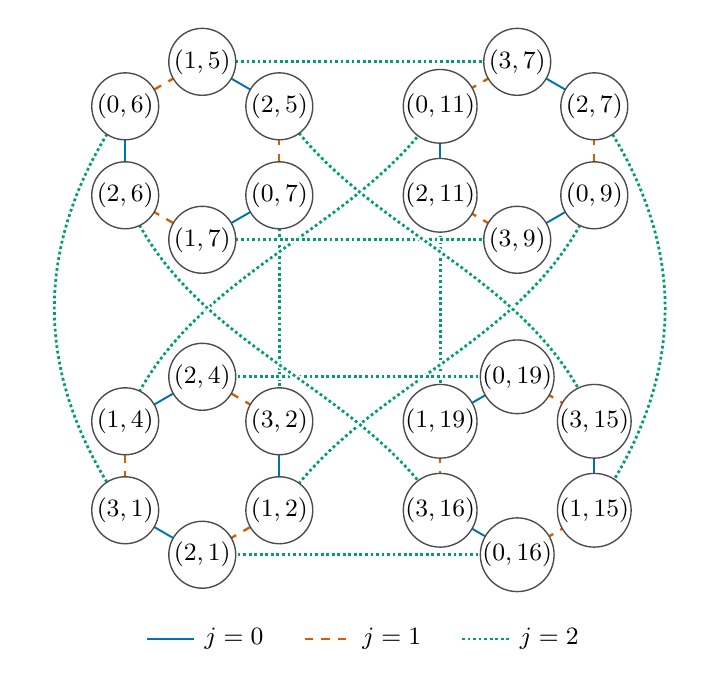
\begin{tikzpicture}[x=1cm,y=1cm,
  g0/.style={exampleJzero,line width=0.7pt},
  g1/.style={exampleJone,dashed,line width=0.85pt},
  g2/.style={exampleJtwo,densely dotted,line width=1pt,preaction={draw=white,solid,line width=2.2pt}},
  vertex/.style={circle,draw=black!70,line width=0.5pt,fill=white,minimum size=8.5mm,inner sep=0pt,font=\small}]
\coordinate (v0) at (-2.97861,2.56500);
\coordinate (v1) at (-1.02139,1.43500);
\coordinate (v2) at (2.97861,1.43500);
\coordinate (v3) at (1.02139,2.56500);
\coordinate (v4) at (2.00000,-3.13000);
\coordinate (v5) at (2.00000,-0.87000);
\coordinate (v6) at (-1.02139,-2.56500);
\coordinate (v7) at (-2.97861,-1.43500);
\coordinate (v8) at (-2.00000,3.13000);
\coordinate (v9) at (-2.00000,0.87000);
\coordinate (v10) at (2.97861,-2.56500);
\coordinate (v11) at (1.02139,-1.43500);
\coordinate (v12) at (-2.00000,-3.13000);
\coordinate (v13) at (-2.00000,-0.87000);
\coordinate (v14) at (-1.02139,2.56500);
\coordinate (v15) at (-2.97861,1.43500);
\coordinate (v16) at (2.97861,2.56500);
\coordinate (v17) at (1.02139,1.43500);
\coordinate (v18) at (-2.97861,-2.56500);
\coordinate (v19) at (-1.02139,-1.43500);
\coordinate (v20) at (2.00000,3.13000);
\coordinate (v21) at (2.00000,0.87000);
\coordinate (v22) at (2.97861,-1.43500);
\coordinate (v23) at (1.02139,-2.56500);
\draw[g0] (v12) -- (v18);
\draw[g0] (v6) -- (v19);
\draw[g0] (v7) -- (v13);
\draw[g0] (v8) -- (v14);
\draw[g0] (v0) -- (v15);
\draw[g0] (v1) -- (v9);
\draw[g0] (v16) -- (v20);
\draw[g0] (v2) -- (v21);
\draw[g0] (v3) -- (v17);
\draw[g0] (v10) -- (v22);
\draw[g0] (v4) -- (v23);
\draw[g0] (v5) -- (v11);
\draw[g1] (v6) -- (v12);
\draw[g1] (v7) -- (v18);
\draw[g1] (v0) -- (v8);
\draw[g1] (v13) -- (v19);
\draw[g1] (v1) -- (v14);
\draw[g1] (v9) -- (v15);
\draw[g1] (v2) -- (v16);
\draw[g1] (v3) -- (v20);
\draw[g1] (v17) -- (v21);
\draw[g1] (v4) -- (v10);
\draw[g1] (v5) -- (v22);
\draw[g1] (v11) -- (v23);
\draw[g2] (v11) -- (v17);
\draw[g2] (v0) .. controls (-4.17861,0.85500) and (-4.17861,-0.85500) .. (v18);
\draw[g2] (v1) -- (v19);
\draw[g2] (v2) .. controls (2.21096,-0.46402) and (0.02910,-0.94882) .. (v6);
\draw[g2] (v3) .. controls (-0.02910,0.94882) and (-2.21096,0.46402) .. (v7);
\draw[g2] (v8) -- (v20);
\draw[g2] (v9) -- (v21);
\draw[g2] (v4) -- (v12);
\draw[g2] (v5) -- (v13);
\draw[g2] (v14) .. controls (0.02910,0.94882) and (2.21096,0.46402) .. (v22);
\draw[g2] (v15) .. controls (-2.21096,-0.46402) and (-0.02910,-0.94882) .. (v23);
\draw[g2] (v10) .. controls (4.17861,-0.85500) and (4.17861,0.85500) .. (v16);
\node[vertex] at (v0) {$(0,6)$};
\node[vertex] at (v1) {$(0,7)$};
\node[vertex] at (v2) {$(0,9)$};
\node[vertex] at (v3) {$(0,11)$};
\node[vertex] at (v4) {$(0,16)$};
\node[vertex] at (v5) {$(0,19)$};
\node[vertex] at (v6) {$(1,2)$};
\node[vertex] at (v7) {$(1,4)$};
\node[vertex] at (v8) {$(1,5)$};
\node[vertex] at (v9) {$(1,7)$};
\node[vertex] at (v10) {$(1,15)$};
\node[vertex] at (v11) {$(1,19)$};
\node[vertex] at (v12) {$(2,1)$};
\node[vertex] at (v13) {$(2,4)$};
\node[vertex] at (v14) {$(2,5)$};
\node[vertex] at (v15) {$(2,6)$};
\node[vertex] at (v16) {$(2,7)$};
\node[vertex] at (v17) {$(2,11)$};
\node[vertex] at (v18) {$(3,1)$};
\node[vertex] at (v19) {$(3,2)$};
\node[vertex] at (v20) {$(3,7)$};
\node[vertex] at (v21) {$(3,9)$};
\node[vertex] at (v22) {$(3,15)$};
\node[vertex] at (v23) {$(3,16)$};
\draw[g0] (-2.7,-4.2) -- (-2.1,-4.2) node[right,black,font=\small] {$j=0$};
\draw[g1] (-0.7,-4.2) -- (-0.09999999999999998,-4.2) node[right,black,font=\small] {$j=1$};
\draw[g2] (1.3,-4.2) -- (1.9,-4.2) node[right,black,font=\small] {$j=2$};
\end{tikzpicture}
